\spacing{1.25}
En este capítulo se presentan los resultados de las simulaciones de chubascos iniciados por rayos cósmicos de energías entre $10^{17}$ y $10^{20}$ eV, considerando tres composiciones primarias, (a) composición ligera, únicamente de protones; (b) composición pesada, únicamente de núcleos de hierro; y (c) composición mixta, de protones y núcleos de helio, nitrógeno y hierro, basada en datos del Observatorio Pierre Auger. Se muestran y discuten resultados de la profundidad del máximo, la distribución lateral de electrones y muones y la densidad de electrones y muones a 1000 m del eje del chubasco. Además se comparan los resultados obtenidos con los tres modelos de interacción hadrónica utilizados para las simulaciones. \\


%\section{Profundidad del máximo $X_{max}$}
%\ccnote{Introducir la sección aclarando que estoy reproduciendo resultados ya conocidos. Citar a PAO y a Sciutto.}
%\subsection{Comparación de predicciones de los modelos hadrónicos}
%Se calculó el promedio de la profundidad del máximo de 100 eventos para cada energía realizando el correspondiente ajuste mediante el algoritmo de mínimos cuadrados no lineal Levenberg-Marquardt. En la gráfica de la Fig. \ref{fig:Xmodelos} se muestran los resultados de $X_{max}$ para los tres modelos hadrónicos.\\
%
%\begin{figure}[h]
%\centering
%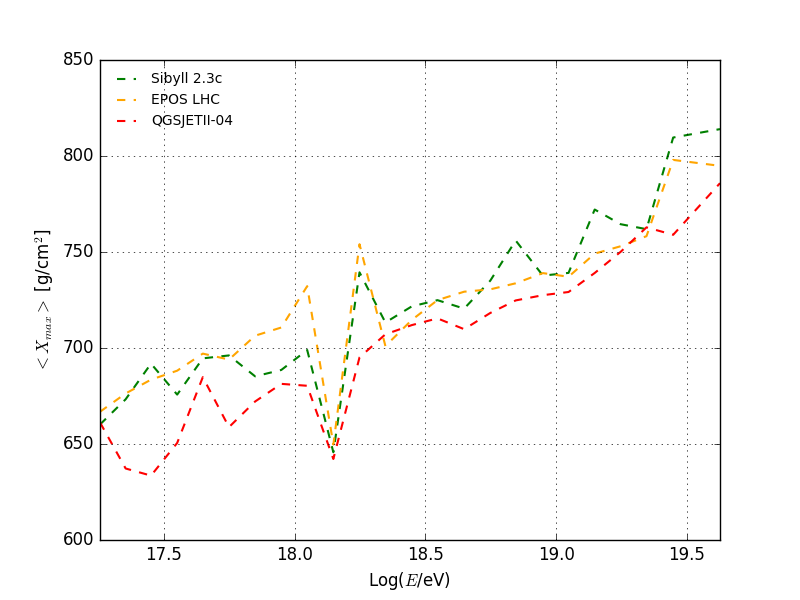
\includegraphics[width=0.7\textwidth]{Figuras/Xmax_modelos} 
%\caption{$X_{max}$ promedio resultante de las simulaciones con los modelos hadrónicos Sibyll 2.3c, EPOS-LHC y QGSJETII-04}
%\label{fig:Xmodelos}
%\end{figure}	
%
%Se observa que en general los tres modelos muestran la misma tendencia de crecimiento de $X_{max}$ con la energía, sin embargo el modelo QGSJET es el que más difiere de los otros dos modelos, prediciendo el máximo a una menor profundidad, con una diferencia promedio de aproximadamente 3\%, mientras que Sibyll y EPOS difieren entre ellos un 1.5\% en promedio.
%
%\begin{table}[h]
%\centering
%\caption{Diferencias porcentuales entre los resultados de $X_{max}$ de los distintos modelos de interacción hadrónica.}
%\begin{tabular}{l|ccc}
%\hline
%              & \multicolumn{1}{l}{Dif. media (\%)} & \multicolumn{1}{l}{Mín. (\%)} & \multicolumn{1}{l}{Máx. (\%)} \\ \hline
%Sibyll/QGSJET & 2.914                               & 0.123                         & 9.207                         \\ \hline
%EPOS/QGSJET   & 3.085                               & 0.379                         & 8.484                         \\ \hline
%Sibyll/EPOS   & 1.473                               & 0.003                         & 4.544  						  \\ \hline 
%\end{tabular}
%\label{modeldif} 
%\end{table}
%
%\subsection{Comparación con datos observacionales}
%En la figura Fig. \ref{fig:Xobs} se muestran tanto los resultados de las simulaciones como los datos obtenidos por el Observatorio Pierre Auger. Los modelos Sibyll y EPOS muestran excelente concordancia con las observaciones en las energías más bajas del rango considerado, luego de $E\approx 10^{18.248}$ eV los datos simulados son en general menores que los experimentales. Por otro lado, QGSJET tiende a subestimar la profundidad del máximo de los chubascos en todo el rango de energías.\\
%
%\begin{figure}[h]
%\centering
%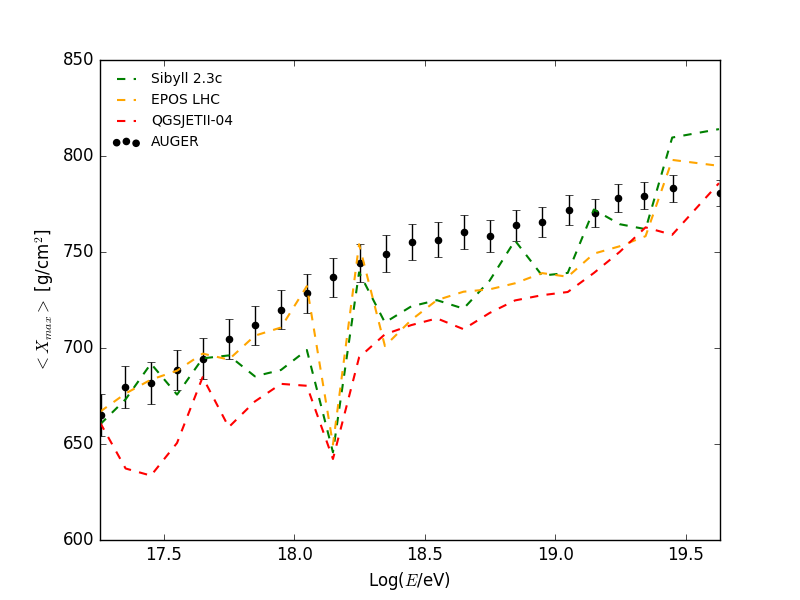
\includegraphics[width=0.7\textwidth]{Figuras/Xmax_modelos_obs} 
%\caption{$X_{max}$ promedio resultante de las simulaciones con los modelos hadrónicos Sibyll 2.3c, EPOS-LHC y QGSJETII-04 junto con los datos tomados por el Observatorio Pierre Auger. Las barras representan el error sisteático de las medidas.}
%\label{fig:Xobs}
%\end{figure}	
%
%Para toda la ventana de energías, el modelo EPOS es el que mejor reproduce los datos del Pierre Auger, con un error relativo de 2.8\% en promedio, le sigue Sibyll con 3.1\% y por último está QGSJET con 5.1\% de error relativo.\\
%
%\begin{table}[h]
%\centering
%\caption{Error porcentual de los resultados de $X_{max}$ de las simulaciones relativo a los datos observacionales.}
%\begin{tabular}{l|ccc}
%\hline
%Modelo & Err. relativo (\%) & Mín. (\%) & Máx. (\%) \\ \hline
%Sibyll & 3.080              & 0.023     & 12.364    \\ \hline
%EPOS   & 2.778              & 0.050     & 11.820    \\ \hline
%QGSJET & 5.092              & 0.589     & 12.840    \\ \hline
%\end{tabular}
%\end{table}
%
%La subestimación de $X_{max}$ en las simulaciones puede sugerir que en las mayores energías, los chubascos se producen por rayos cósmicos de composición más ligera que la que se ha considerado. Sin embargo, como evidencian las discrepancias entre los modelos, la reproducción de los datos observacionales es altamente dependiente del modelo hadrónico utilizado y de sus características particulares.


%%% Resultados de Xmax
\section{Efecto de la composición primaria en la profundidad del máximo}
A partir de las simulaciones realizadas con la metodología antes expuesta, a manera de validación se calculó la profundidad del máximo promedio $\langle X_{\text{max}} \rangle$ para cada subintervalo de energía. En la figura \ref{fig:xmax_pfe} se muestran los ajustes lineales de la forma
\begin{align}
\langle X_{\text{max}} \rangle = \Lambda \log E + c,
\end{align}

realizados a los datos obtenidos de las simulaciones de chubascos con composición constante.\\

\begin{figure}[]
\centering
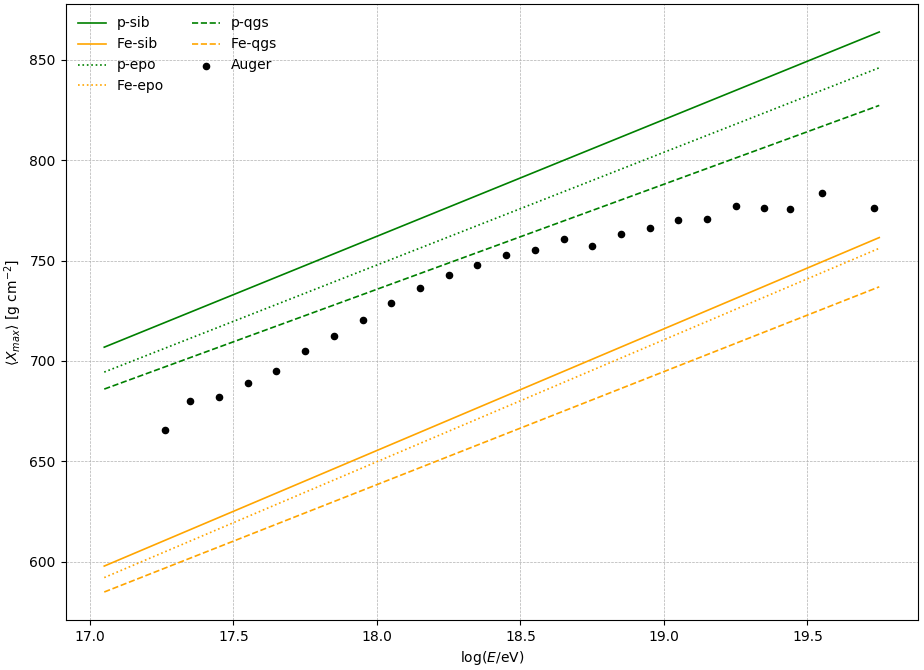
\includegraphics[width=0.8\textwidth]{Figuras/Xmax_pFe_fit.png}
\caption{Resultados del ajuste lineal de los datos de profundidad del máximo obtenidos de simulaciones de chubascos de ultraalta energía.}
\label{fig:xmax_pfe}
\end{figure}

En general los resultados de esta observable para chubascos producidos por protones (p) y núcleos de hierro (Fe) coinciden con el modelo analítico Heitler-Matthews, que para chubascos producidos por protones predice una tasa de elongación $\Lambda = 58 \text{ g/cm}^2$. Asimismo, las diferencias entre los resultados de los modelos hadrónicos mostrados en la figura concuerdan con los resultados reportados por diferentes autores \cite{Heck2003,Pierog2018,Bellido2017} que han utilizado otros programas de simulación y más variantes de los modelos. Los parámetros obtenidos del ajuste lineal para cada uno de los modelos se muestran en la tabla \ref{linear_params} \\

\begin{table}[] 
\centering
\caption{Parámetros del ajuste lineal a los datos de $X_{\text{max}}$ de diferentes modelos y composiciones}
\begin{tabular}{c|c|cc}
\hline
Modelo                       &  Prim  	& $\Lambda$ 	& $b$      \\ \hline
\multirow{2}{*}{Sibyll 2.3c} & 	p  		& 58.133    	& -284.299 \\  
                             & 	Fe 		& 60.589    	& -435.177 \\ \hline
\multirow{2}{*}{EPOS-LHC}    & 	p  		& 56.129    	& -262.527 \\  
                             & 	Fe 		& 60.731    	& -443.335 \\ \hline
\multirow{2}{*}{QGSJETII-04} & 	p  		& 52.319    	& -206.041 \\ 
                             & 	Fe 		& 56.287    	& -374.749 \\ \hline
\end{tabular}
\label{linear_params}
\end{table}

Como se explica en \cite{Pierog2018}, el modelo Sibyll 2.3c predice mayores valores de $\langle X_{\text{max}} \rangle$ debido a la baja multiplicidad y alta elasticidad considerada para las interacciones, y por el otro lado QGSJETII-04 predice los valores más bajos ya que considera la multiplicidad más alta y una sección eficaz baja en interacciones con núcleos del aire.\\

En la figura \ref{fig:xmax_mix} se muestran los resultados de las simulaciones con composición primaria mixta, así como los datos obtenidos por el PAO. Los modelos Sibyll 2.3c y EPOS-LHC muestran buena concordancia con las observaciones en las energías más bajas del rango considerado, luego de $E\approx 10^{18.3}$ eV los datos simulados son en general menores que los experimentales. Por otro lado, QGSJETII-04 tiende a subestimar la profundidad del máximo de los chubascos en todo el rango de energías.\\

\begin{figure}[] 
\centering
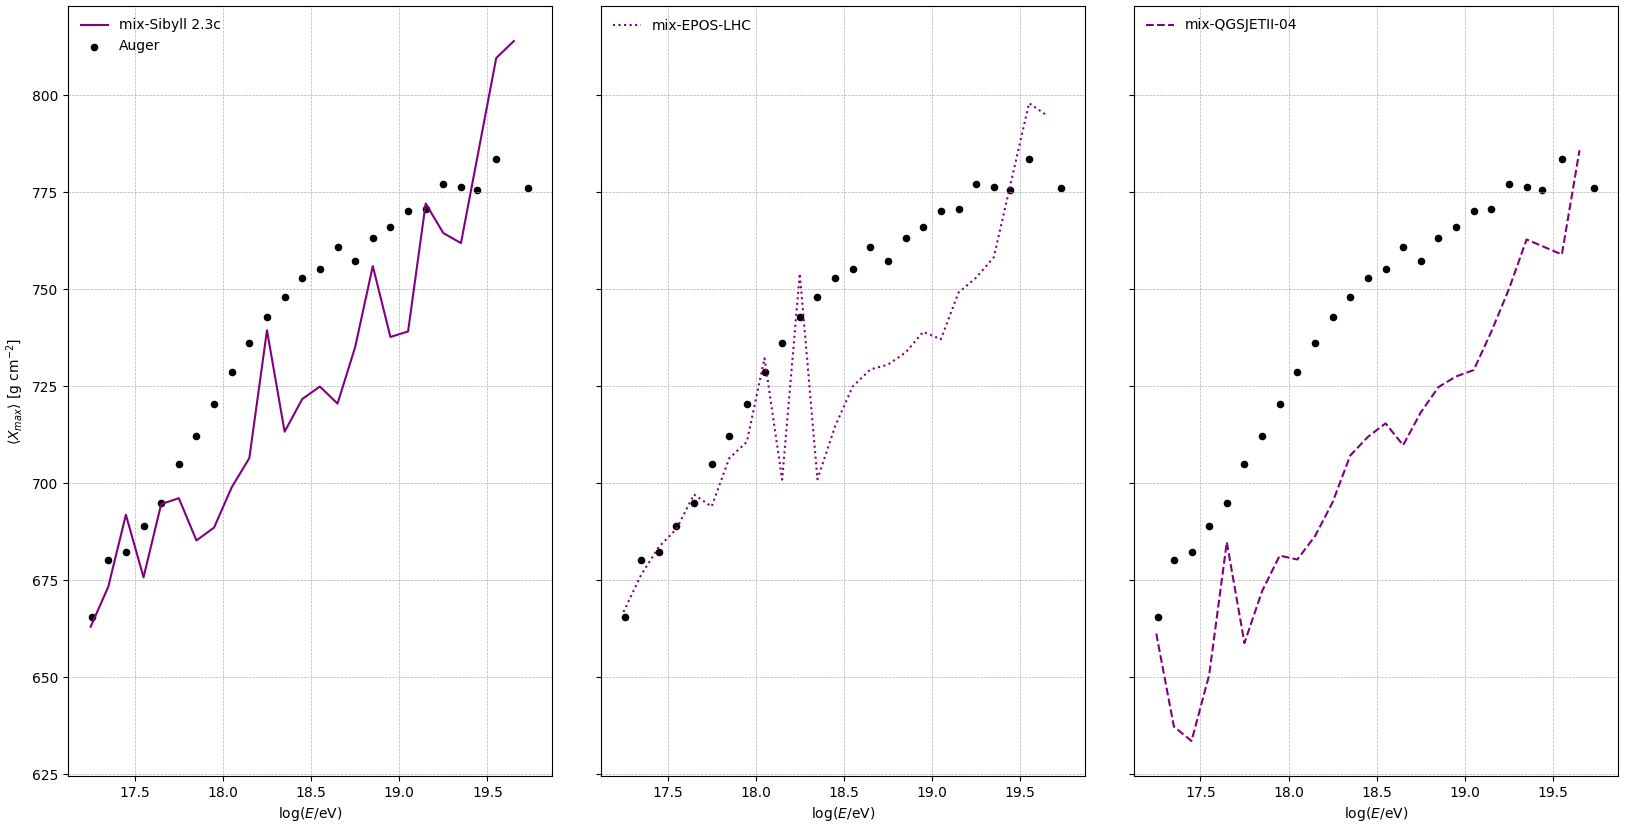
\includegraphics[width=\textwidth]{Figuras/Xmax_mix}
\caption{Resultados de la profundidad del máximo en chubascos con composición primaria mixta, comparándolos con datos experimentales del Observatorio Pierre Auger.}
\label{fig:xmax_mix}
\end{figure}

Considerando el intervalo de energías completo, el modelo EPOS-LHC es el que mejor reproduce los datos del Pierre Auger con un error relativo de 2.8\% en promedio, le sigue Sibyll 2.3c con 3.1\% y por último está QGSJETII-04 con 5.1\% de error relativo.\\

\begin{table}[h]
\centering
\caption{Error porcentual de los resultados de $X_{max}$ de las simulaciones relativo a los datos observacionales.}
\begin{tabular}{c|ccc}

Modelo & Err. relativo (\%) & Mín. (\%) & Máx. (\%) \\ \hline
Sibyll 2.3c 	& 3.080              & 0.023     & 12.364    \\ \hline
EPOS-LHC   		& 2.778              & 0.050     & 11.820    \\ \hline
QGSJETII-04 	& 5.092              & 0.589     & 12.840    \\ \hline
\end{tabular}
\end{table}

%%% Resultados de distribuciones laterales 
\section{Distribuciones laterales de electrones y muones}
Se presentan las distribuciones laterales resultantes de los chubascos en el intervalo de energía completo, así como de ciertos subintervalos. Se calculó la densidad de electrones y muones separadamente. Cada distribución se ha ajustado a una función NKG modificada \cite{Gaisser2016} de la forma
\begin{align} \label{modifiedNKG}
\rho (r) = c \qty(\frac{r}{r_{opt}})^{-\beta}\qty(1-\frac{r}{r_{opt}})^{-\beta},
\end{align}
donde $c$ representa una medida de la densidad de partículas a una distancia $r_{opt} = 1000$ m y $\beta$ representa la pendiente de la distribución, ambos son parámetros libres. Se ha elegido el valor de $r_{\text{opt}}$ de acuerdo al valor de la distancia óptima \cite{Newton2007} según las características del sitio de las simulaciones (el Observatorio Pierre Auger).

%	\begin{itemize}
%	\item Qué resultados se van a presentar
%	\item Describir los ajustes y las FDL y citar la fuente de cada una.
%	\item Adelantar cuál modelo es mejor (si se puede)
%	\item Adelantar cuál es el efecto de la composición
%	\end{itemize}

	\subsection{Resultados de todo el intervalo de energía}
	En la figura \ref{fig:distlat} se muestran la distribuciones laterales de electrones y muones	producidos en chubascos de p y Fe. Se muestran los resultados de las simulaciones con los diferentes modelos. Los parámetros del ajuste de la función (\ref{modifiedNKG}) para los tres modelos se presentan en las tablas \ref{edistlat_params} y \ref{mudistlat_params}. Se observa que para todos los modelos y partículas primarias los electrones muestran una mayor pendiente en su distribución, dada por el parámetro $\beta$. \\
	
\begin{figure}[ht] 
\centering
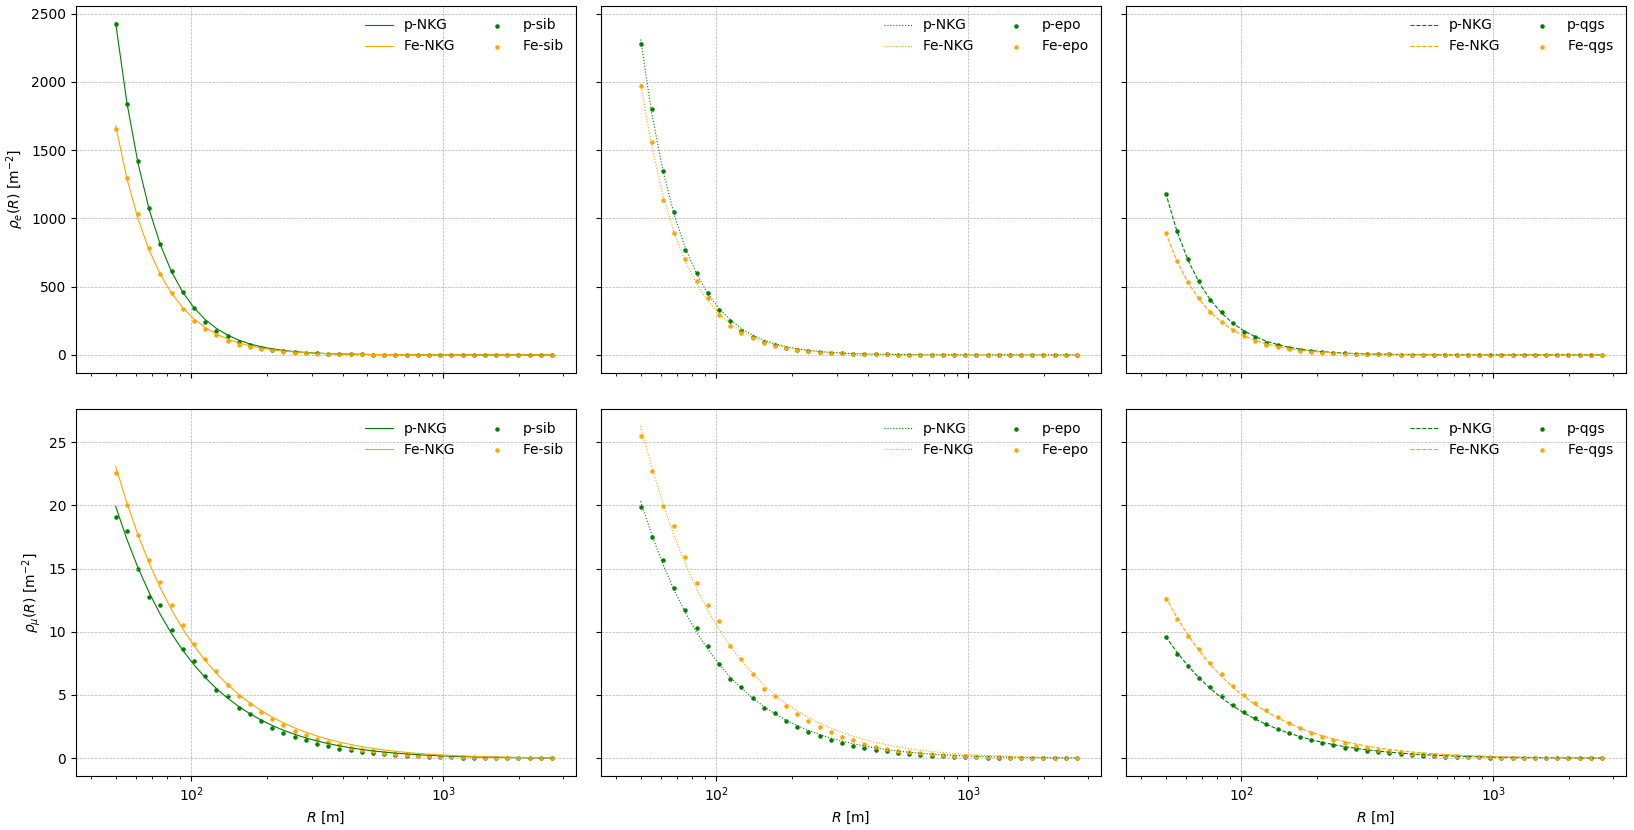
\includegraphics[width=\textwidth]{Figuras/distlat_pFe}
\caption{\textit{Fila superior}: distribuciones laterales de electrones. \textit{Fila inferior}: distribuciones laterales de muones. Distribuciones resultado de chubascos en todo el rango de energías considerado. Cada columna muestra resultados de un modelo hadrónico.}
\label{fig:distlat}
\end{figure}
		
\begin{table}[ht] 
\centering
\caption{Parámetros del ajuste de la distribución lateral de electrones a la función (\ref{modifiedNKG}).}
\begin{tabular}{c|c|cc}
Modelo                       & Prim. & $c$   & $\beta$ \\ \hline
\multirow{2}{*}{Sibyll 2.3c} & p     & 1.313 & 2.553   \\
                             & Fe    & 1.339 & 2.421   \\ \hline
\multirow{2}{*}{EPOS-LHC}    & p     & 1.437 & 2.505   \\
                             & Fe    & 1.390 & 2.465   \\ \hline
\multirow{2}{*}{QGSJETII-04} & p     & 0.757 & 2.497   \\
                             & Fe    & 0.691 & 2.432   \\ \hline
\end{tabular}
\label{edistlat_params}
\end{table}

\begin{table}[] 
\centering
\caption{Parámetros del ajuste de la distribución lateral de muones a la función (\ref{modifiedNKG}).}
\begin{tabular}{c|c|cc}
Modelo                       & Prim. & $c$   & $\beta$ \\ \hline
\multirow{2}{*}{Sibyll 2.3c} & p     & 0.436 & 1.297   \\
                             & Fe    & 0.586 & 1.247   \\ \hline
\multirow{2}{*}{EPOS-LHC}    & p     & 0.425 & 1.313   \\
                             & Fe    & 0.684 & 1.238   \\ \hline
\multirow{2}{*}{QGSJETII-04} & p     & 0.212 & 1.295   \\
                             & Fe    & 0.318 & 1.253   \\ \hline
\end{tabular}
\label{mudistlat_params}
\end{table}

	Los tres modelos de interacciones hadrónicas de altas energías muestran el mismo comportamiento en la forma de las distribuciones, sin embargo es evidente que QGSJETII-04 predice una menor densidad de partículas en todo el rango de $R$, el parámetro $c$ indica que en general a nivel del suelo estarían llegando la mitad de partículas que con respecto a los otros dos modelos, como también se evidencia en la figura \ref{fig:distlat_modelos}, donde se han graficado las razones de las densidades predichas por los diferentes modelos. Una vez más, esto se atribuye a la baja multiplicidad de partículas del modelo a comparación de los otros; si durante el chubasco se producen menos piones neutros y cargados, o menos mesones en general, consecuentemente se producirán menos electrones y muones de sus respectivos decaimientos. \\
	
\begin{figure}[] 
\centering
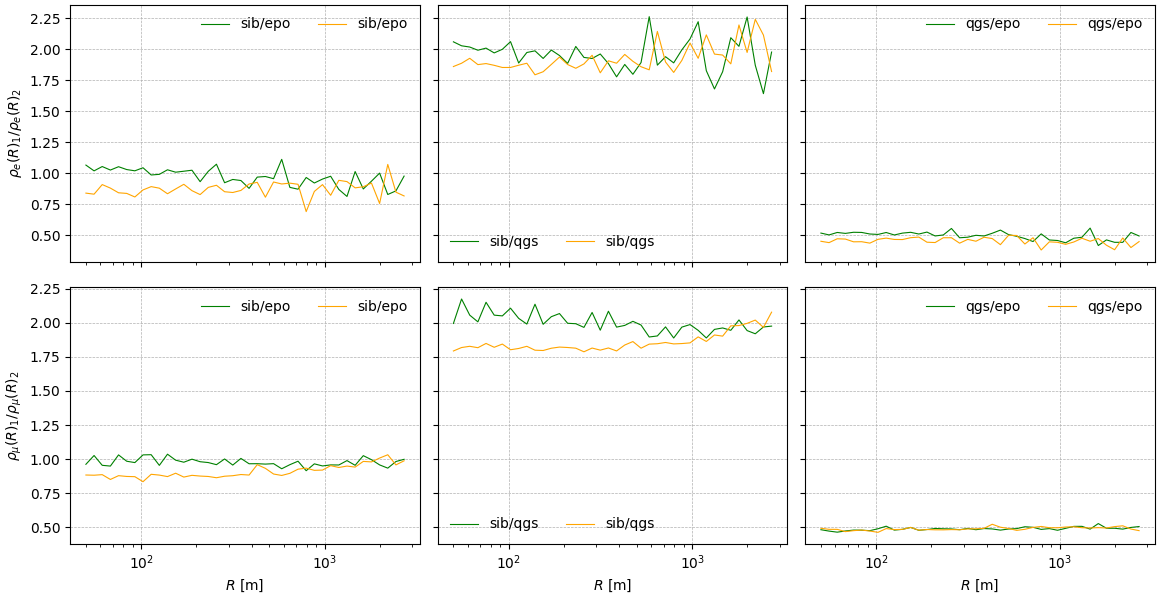
\includegraphics[width=\textwidth]{Figuras/distlat_models}
\caption{Razones entre densidades de partículas de pares de modelos de interacción hadrónica.}
\label{fig:distlat_modelos}
\end{figure}

Respecto a la composición primaria se observa que las diferencias entre las distribuciones son significativas únicamente a cortas distancias, en las cuales se producen más electrones en los chubascos de protones y más muones en los de núcleos de hierro. En el rango completo de $R$, los parámetros del ajuste presentan pequeñas diferencias del orden de $10^{-1}$ y $10^{-2}$.
	
	\subsection{Resultados de algunos subintervalos}
	Se graficaron las distribuciones laterales para tres subintervalos de energía designados como $bin02$, $bin13$ y $bin24$, con energías
\begin{align*}
10^{17.1} \leq & E_{bin03} < 10^{17.2} \text{ eV}, \\
10^{18.2} \leq & E_{bin14} < 10^{18.3} \text{ eV}, \text{ y}\\
10^{19.7} \leq & E_{bin23} < 10^{19.8} \text{ eV}
\end{align*}	
	 respectivamente. En las figuras \ref{fig:distlat_bin02}, \ref{fig:distlat_bin13} y \ref{fig:distlat_bin24} se muestran las distribuciones de electrones y las de muones para cada subintervalo. Cada una se ajustó a la función (\ref{modifiedNKG}) cuyos parámetros se encuentran en las tablas \ref{edistlat_binparams} y \ref{mudistlat_binparams}. \\

\begin{figure}[h] 
\centering
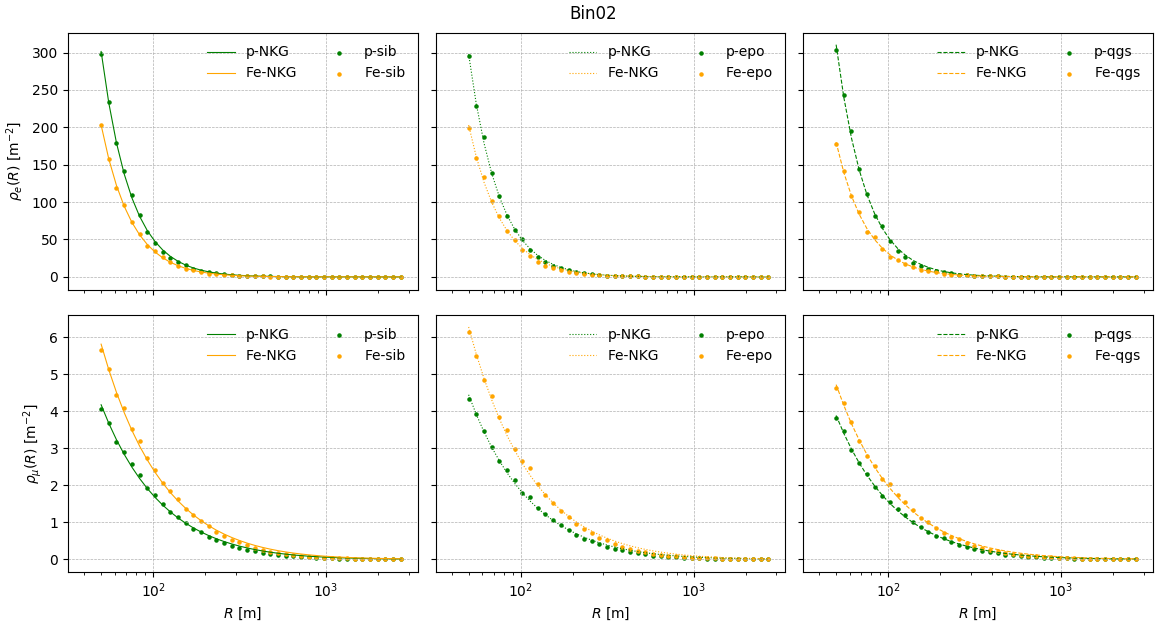
\includegraphics[width=\textwidth]{Figuras/distlat_bin02}
\caption{Distribuciones laterales de electrones y muones resultado de chubascos de energía promedio $E=10^{17.15}$ eV.}
\label{fig:distlat_bin02}
\end{figure}

\begin{figure}[] 
\centering
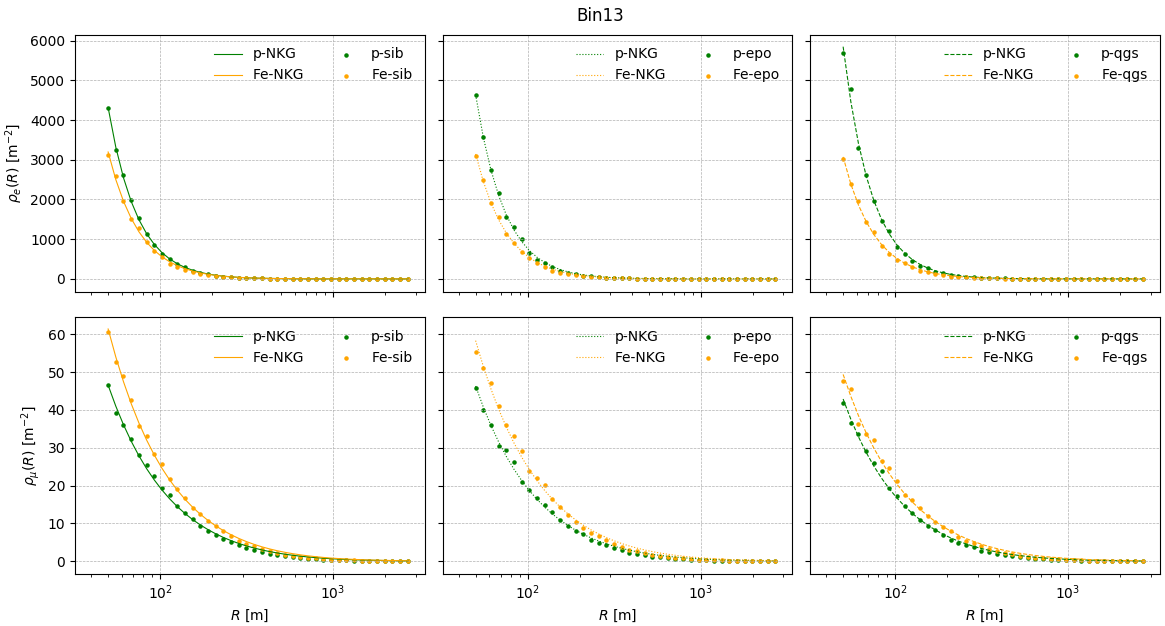
\includegraphics[width=\textwidth]{Figuras/distlat_bin13}
\caption{Distribuciones laterales de electrones y muones resultado de chubascos de energía promedio $E=10^{18.25}$ eV.}
\label{fig:distlat_bin13}
\end{figure}

\begin{figure}[] 
\centering
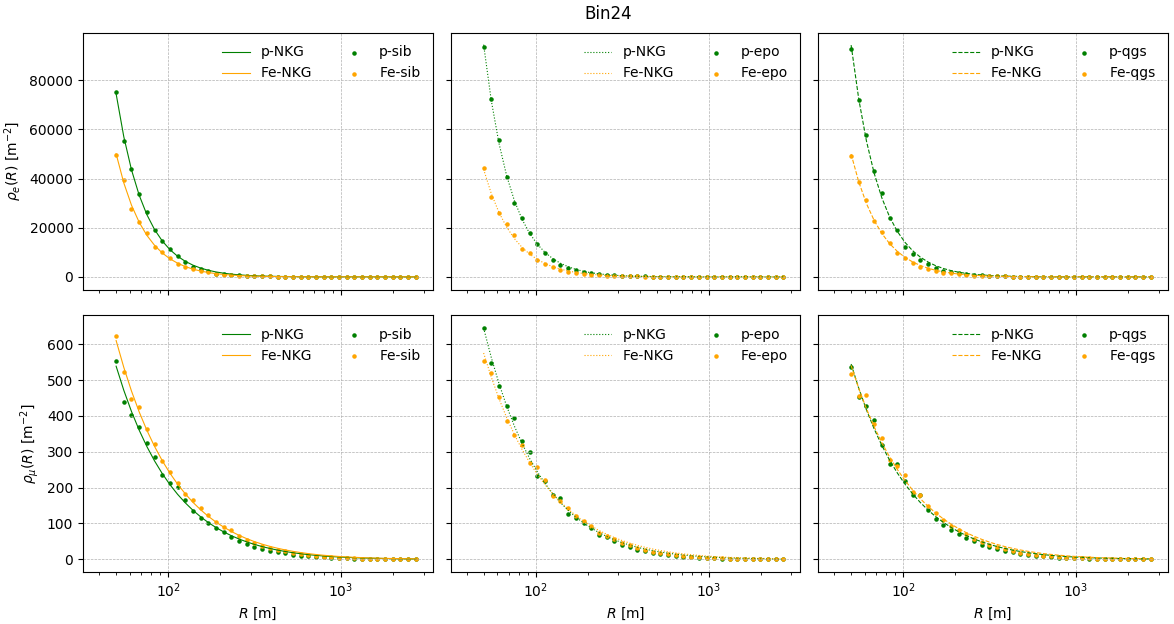
\includegraphics[width=\textwidth]{Figuras/distlat_bin24}
\caption{Distribuciones laterales de electrones y muones resultado de chubascos de energía promedio $E=10^{19.75}$ eV.}
\label{fig:distlat_bin24}
\end{figure}

Considerando la evolución de las distribuciones con la energía primaria, en general el número de partículas llegando al suelo por metro cuadrado aumenta considerablemente, como se esperaba debido al aumento de la producción de partículas con la energía. Además cabe mencionar que las diferencias entre la forma de las distribuciones de electrones y muones en los subintervalos se mantiene similar a la observada en el rango completo. No obstante, para energías individuales no se manifiesta una discrepancia notoria entre los tres modelos hadrónicos.\\

Particularmente en la distribución de muones puede verse que a medida aumenta la energía inicial, los chubascos producidos por p y Fe se vuelven prácticamente indistinguibles, por lo que éstas no serían útiles para dilucidad la masa de la partícula primaria. En el caso de los electrones se observa lo contrario, las diferencias en el parámetro $c$ para el último subintervalo entre p y Fe es mayor que a energías menores. \\

\begin{table}[] 
\centering
\caption{Parámetros del ajuste de la distribución lateral de electrones a la función (\ref{modifiedNKG}) para tres subintervalos de energía.}
\begin{tabular}{cc|cc|cc|cc}
\hline
\multicolumn{2}{c|}{Subintervalo}                          & \multicolumn{2}{c|}{$bin02$} & \multicolumn{2}{c|}{$bin13$} & \multicolumn{2}{c}{$bin24$} \\ \hline
\multicolumn{1}{c|}{Modelo}                       & Prim. & $c$          & $\beta$       & $c$          & $\beta$       & $c$          & $\beta$       \\ \hline
\multicolumn{1}{c|}{\multirow{2}{*}{Sibyll 2.3c}} & p     & 0.242        & 2.419         & 3.154        & 2.450         & 48.247       & 2.491         \\
\multicolumn{1}{c|}{}                             & Fe    & 0.193        & 2.362         & 3.811        & 2.284         & 30.944       & 2.507         \\ \hline
\multicolumn{1}{c|}{\multirow{2}{*}{EPOS-LHC}}    & p     & 0.282        & 2.362         & 3.433        & 2.446         & 48.576       & 2.570         \\
\multicolumn{1}{c|}{}                             & Fe    & 0.319        & 2.191         & 3.423        & 2.315         & 38.819       & 2.385         \\ \hline
\multicolumn{1}{c|}{\multirow{2}{*}{QGSJETII-04}} & p     & 0.270        & 2.392         & 3.577        & 2.511         & 61.917       & 2.487         \\
\multicolumn{1}{c|}{}                             & Fe    & 0.171        & 2.361         & 3.140        & 2.336         & 42.061       & 2.402         \\ \hline
\end{tabular}
\label{edistlat_binparams}
\end{table}	 

\begin{table}[] 
\centering
\caption{Parámetros del ajuste de la distribución lateral de muones a la función (\ref{modifiedNKG}) para tres subintervalos de energía.}
\begin{tabular}{cc|cc|cc|cc}
\hline
\multicolumn{2}{c|}{Subintervalo}                          & \multicolumn{2}{c|}{$bin02$} & \multicolumn{2}{c|}{$bin13$} & \multicolumn{2}{c}{$bin24$} \\ \hline
\multicolumn{1}{c|}{Modelo}                       & Prim. & $c$          & $\beta$       & $c$          & $\beta$       & $c$          & $\beta$       \\ \hline
\multicolumn{1}{c|}{\multirow{2}{*}{Sibyll 2.3c}} & p     & 0.124        & 1.193         & 1.431        & 1.182         & 13.841       & 1.243         \\
\multicolumn{1}{c|}{}                             & Fe    & 0.179        & 1.181         & 1.811        & 1.196         & 16.816       & 1.219         \\ \hline
\multicolumn{1}{c|}{\multirow{2}{*}{EPOS-LHC}}    & p     & 0.135        & 1.185         & 1.397        & 1.188         & 15.138       & 1.273         \\
\multicolumn{1}{c|}{}                             & Fe    & 0.205        & 1.161         & 1.968        & 1.150         & 18.815       & 1.161         \\ \hline
\multicolumn{1}{c|}{\multirow{2}{*}{QGSJETII-04}} & p     & 0.101        & 1.238         & 1.135        & 1.233         & 13.823       & 1.247         \\
\multicolumn{1}{c|}{}                             & Fe    & 0.147        & 1.178         & 1.622        & 1.159         & 17.012       & 1.174         \\ \hline
\end{tabular}
\label{mudistlat_binparams}
\end{table}
	 

%%% Resultados de densidad de particulas en r=1000 m
\section{Densidad de partículas en $r_{\text{opt}}$}
A continuación se presentan los resultados de la densidad de partículas a la distancia $r_{\text{opt}}=1000$ m del eje del chubasco en función de la energía primaria del mismo. En la figura \ref{fig:density} se muestran los resultados de las simulaciones junto con un ajuste a una función tipo ley de potencias:
\begin{align} \label{powerlaw}
\rho_{r_{opt}(E)} = a \qty(\frac{E}{10^{18}})^b,
\end{align}
donde $a$ y $b$ son parámetros libres. Los resultados de los ajustes se encuentran en las tablas \ref{edensity_params} y \ref{mudensity_params}. \\

\begin{figure}[h] 
\centering
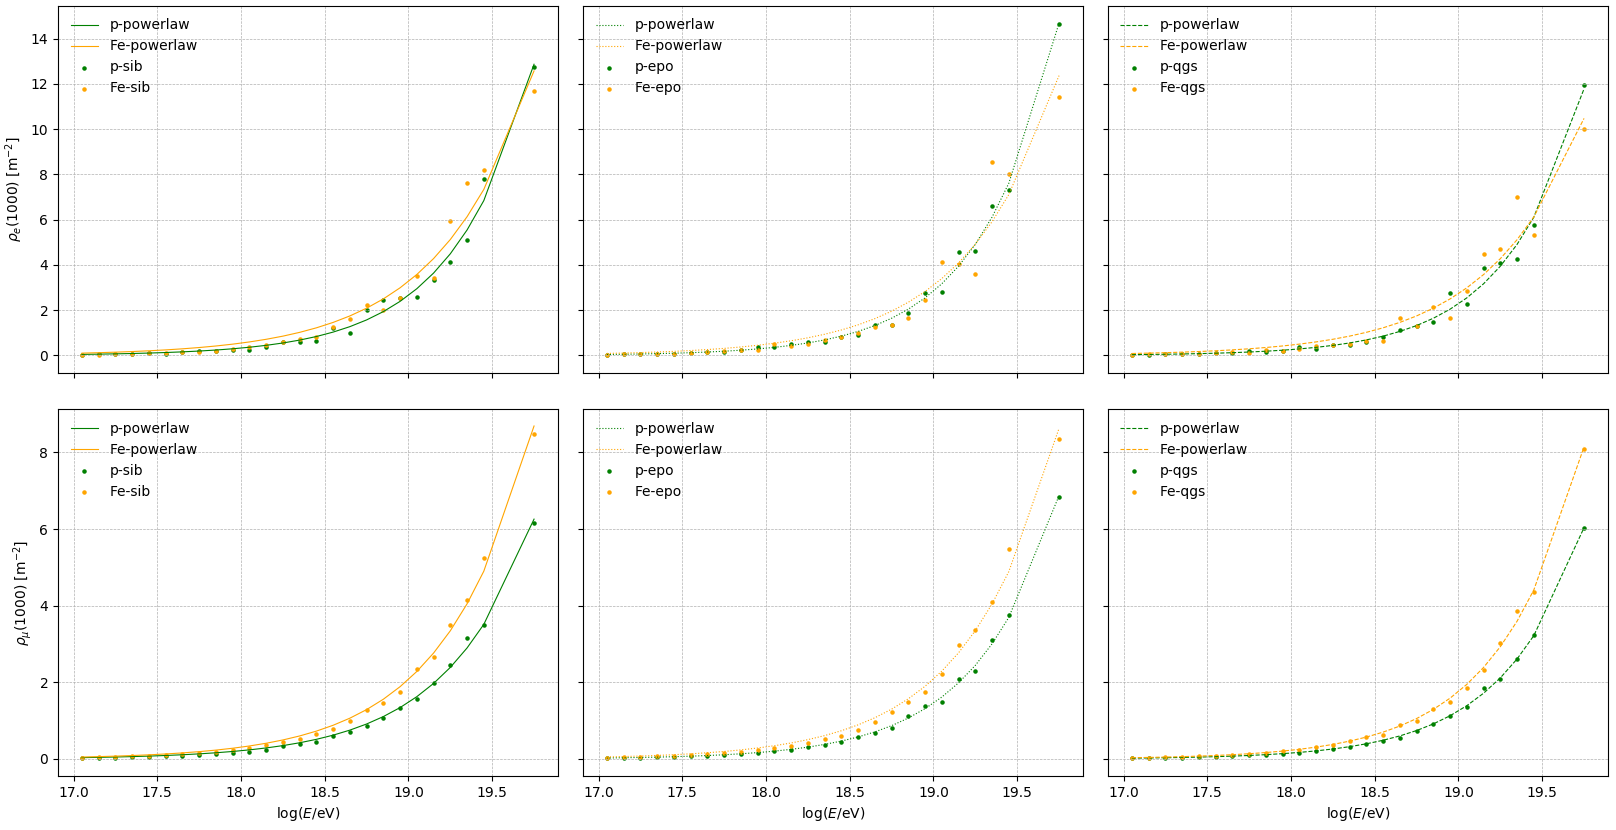
\includegraphics[width=\textwidth]{Figuras/density_pFe}
\caption{Densidad de partículas (electrones y muones) a una distancia $R=r_{opt}$ en función de la energía inicial}
\label{fig:density}
\end{figure}

\begin{table}[] 
\centering
\caption{Parámetros del ajuste de la densidad de electrones a la función (\ref{powerlaw}).}
\begin{tabular}{c|c|cc}
Modelo                       & Prim. & $a$ & $b$   \\ \hline
\multirow{2}{*}{Sibyll 2.3c} & p     & 0.323     & 0.915 \\
                             & Fe    & 0.542     & 0.780 \\ \hline
\multirow{2}{*}{EPOS-LHC}    & p     & 0.317     & 0.952 \\
                             & Fe    & 0.489     & 0.802 \\ \hline
\multirow{2}{*}{QGSJETII-04} & p     & 0.255     & 0.952 \\
                             & Fe    & 0.454     & 0.779 \\ \hline
\end{tabular}
\label{edensity_params}
\end{table}

\begin{table}[] 
\centering
\caption{Parámetros del ajuste de la densidad de muones a la función (\ref{powerlaw}).}
\begin{tabular}{c|c|cc}
Modelo                       & Prim. & $a$ 		 & $b$   \\ \hline
\multirow{2}{*}{Sibyll 2.3c} & p     & 0.215     & 0.836 \\
                             & Fe    & 0.308     & 0.829 \\ \hline
\multirow{2}{*}{EPOS-LHC}    & p     & 0.184     & 0.898 \\
                             & Fe    & 0.314     & 0.822 \\ \hline
\multirow{2}{*}{QGSJETII-04} & p     & 0.154     & 0.911 \\
                             & Fe    & 0.227     & 0.888 \\ \hline
\end{tabular}
\label{mudensity_params}
\end{table}

Se observa que la forma de las funciones, tanto para electrones y muones es bastante similar pero siempre manteniendo un mayor número de electrones en general, tal como en las distribuciones laterales. Por otro lado, no se advierte una dependencia significativa del modelo hadrónico para la densidad a 1000 m, sin embargo la razón entre pares de modelos es bastante fluctuante, como se aprecia en la figura \ref{fig:density_modelos}, aunque en ninguno de los casos el promedio de los valores se aleja demasiado de 1.0; el caso de la cantidad de muones producidos por QGSJETII-04 sigue siendo el más extremo sin llegar a los valores de la figura \ref{fig:distlat_modelos}. \\

\begin{figure}[]
\centering
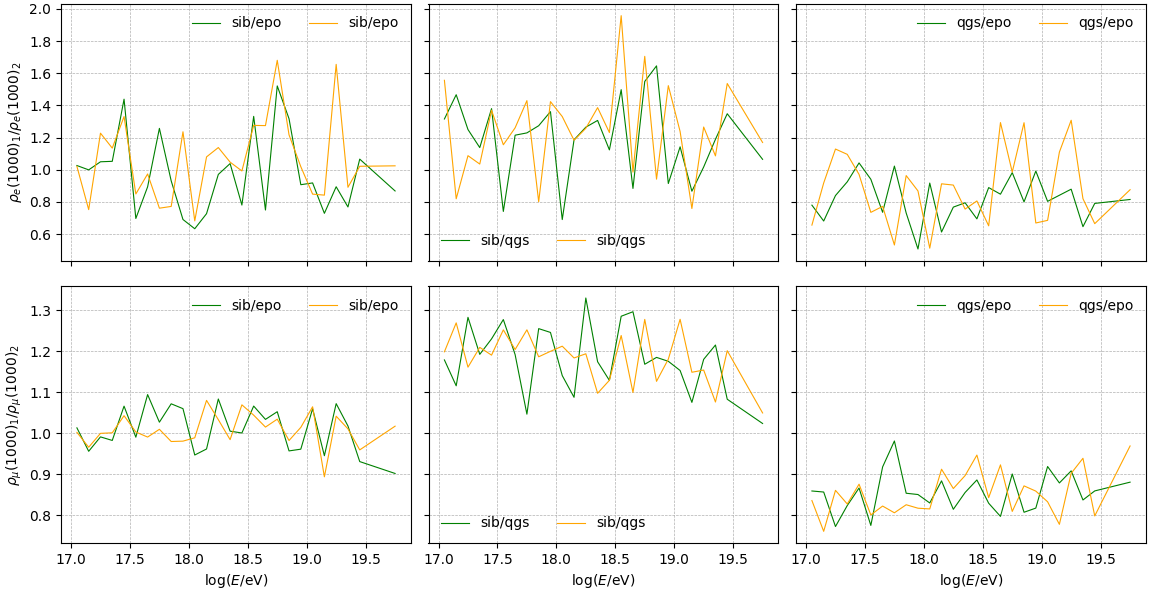
\includegraphics[width=\textwidth]{Figuras/density_models}
\caption{Razones entre densidades de pares de modelos en función de la energía primaria del chubasco.}
\label{fig:density_modelos}
\end{figure}

Adicionalmente, las densidades de electrones en función de la energía primaria no muestra una clara dependencia de la masa de la partícula primaria, siendo que ambas funciones casi se sobreponen. En el caso de los muones, es claro que la diferencia en densidades a 1000 m de chubascos de p y Fe aumenta gradualmente a medida que la energía primaria es mayor. Sin embargo en ambos casos el parámetro $a$, que es una medida de $\rho_{1000}$ a una energía inicial de $10^{18}$ eV, es mayor para chubascos iniciados por Fe y $b$ es consistentemente mayor para chubascos iniciados por protones.

\singlespacing